%!TEX root = main.tex
This block buffers the measurement so that the device is able to drive a \SI{10}{\pico\farad} capacitive load. It is expected to be the primary current consumer of the device ($\sim \SI{200}{\micro\ampere}$).

\subsection{Principle of Operation}
As shown in figure~\ref{fig:buffer},
\begin{figure}
  \centering
  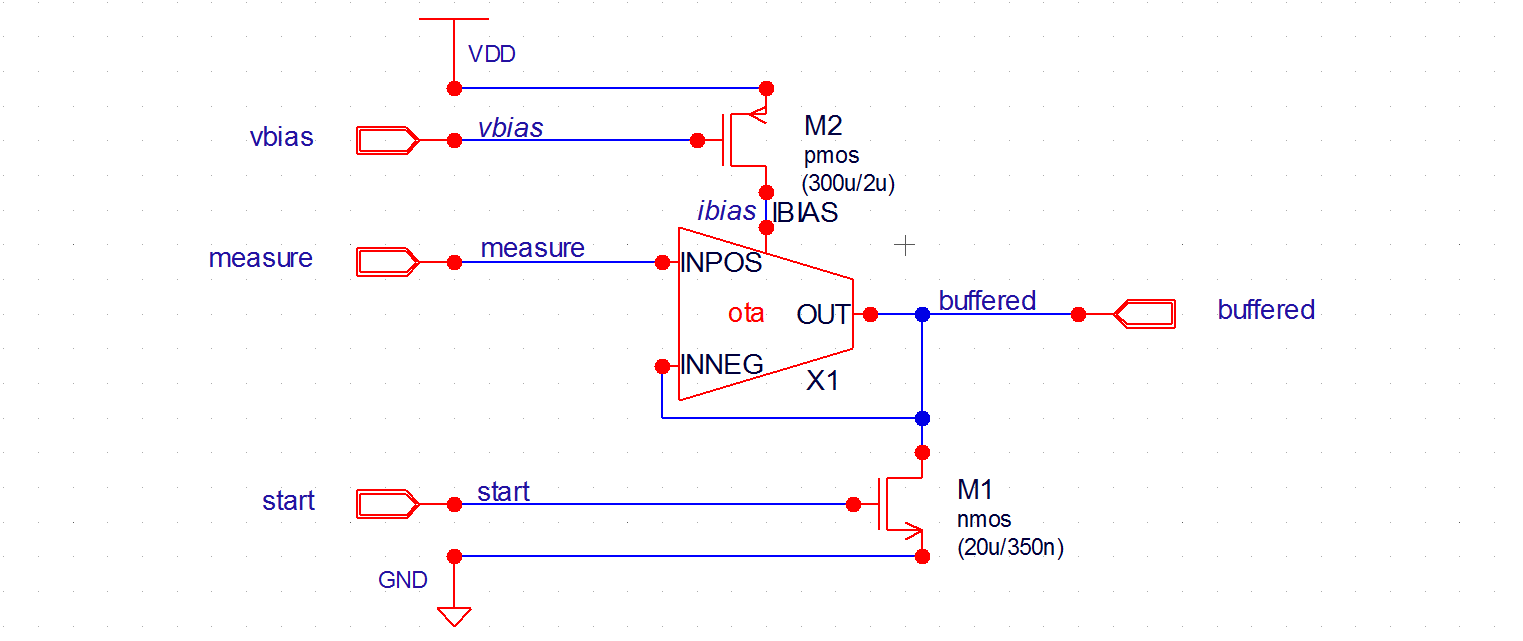
\includegraphics[width=\textwidth]{buffer.png}
  \caption{\blk{buffer} circuit.\label{fig:buffer}}
\end{figure}
\blk{buffer} is made using an OTA in follower configuration.
Similarly to \blk{rampgen}, the output can be shorted by \sig{M1} to ground.
While this would not be necessary if the output stage was built around an ideal amplifier, it allows reduce the specifications on the slew rate of the OTA.
Because we do not care about linearity when resetting the output to ground, this responsibility is left to a minimal length transitor with digital input.
This allows to concentrate on the linearity and the gain\footnote{Follower error $\sim \frac{1}{A_{loop}}$} of the OTA itself which does not need a high slew rate anymore.

\subsection{Sizing}
The OTA is a simple CMOS differential pair. The input stage uses PMOS transistors so that the input range matches the output range of \blk{rampgen}.
The widths are chosen so that the OTA can deliver enough current to drive the specified load. The NMOS loads are \SI{2}{\micro\meter} long in order to reduce their $g_{ds}$. However, the PMOS input transistors are not as long because they would get too wide in order to match the $I_{ds}$. The width required to drive the load is of the order of a couple of hundreds of \si{\micro\meter}.

The OTA bias current is provided by \sig{M2}, which is \SI{2}{\micro\meter} long in order to have a good current source behaviour. It is biased with the same voltage as \blk{rampgen}, which provides a low $V_{ov}$ in order to maximize the output range. It is the largest transistor of the device.

Finally \sig{M1} is of minimum length since linearity is not important during the reset phase, and wide enough to drive the output from \SI{3.3}{\volt} to ground in the length of a pulse, \SI{10}{\nano\second}.
